\documentclass[11pt,a4paper,twoside,openright]{book}

%!TEX root=thesis.tex
\usepackage[
  pdftex,
  plainpages=false,
  colorlinks,
  hyperindex,
  pdfpagemode=UseNone,
  bookmarksopen,
  linkcolor=black,
  citecolor=black,
  urlcolor=black]{hyperref}
\usepackage{graphicx}
\usepackage[boxed]{algorithm}
\usepackage{setspace}
\usepackage{algorithm}
\usepackage{algorithmic}
\usepackage{subfigure}
\usepackage[utf8]{inputenc}
\usepackage[nocompress]{cite}
\usepackage[show]{chato-notes}
\usepackage{booktabs}
\usepackage{enumitem}
\usepackage{amsmath}
\usepackage{mathtools}
\usepackage{url}
\usepackage{listings}
\usepackage{xcolor}

%syntax highlighting for code
\lstset{%
  language=C++,
  basicstyle=\ttfamily,
  keywordstyle=\color{blue}\ttfamily,
  stringstyle=\color{red}\ttfamily,
  commentstyle=\color{green}\ttfamily,
  morecomment=[l][\color{magenta}]{\#}
}

\lstdefinelanguage{XML}{%
  morestring=[b]",
  morestring=[s]{>}{<},
  morecomment=[s]{<?}{?>},
  stringstyle=\color{black},
  identifierstyle=\color{blue},
  keywordstyle=\color{cyan},
  morekeywords={xmlns,version,type}% list your attributes here
}
%end syntax highlighting

\DeclarePairedDelimiter{\ceil}{\lceil}{\rceil}
\graphicspath{{img/}} % Specifies the directory where pictures are stored

\hypersetup{
    unicode=true,          % non-Latin characters in Acrobats bookmarks
    pdftoolbar=true,        % show Acrobats toolbar?
    pdfmenubar=true,        % show Acrobats menu?
    pdffitwindow=false,     % window fit to page when opened
    pdfstartview={FitH},    % fits the width of the page to the window
    pdftitle={My title},    % title
    pdfauthor={Author},     % author
    pdfsubject={Subject},   % subject of the document
    pdfcreator={Creator},   % creator of the document
    pdfproducer={Producer}, % producer of the document
    pdfnewwindow=true,      % links in new window
    colorlinks=true,       % false: boxed links; true: colored links
    linkcolor=black,          % color of internal links
    citecolor=black,        % color of links to bibliography
    filecolor=black,      % color of file links
    urlcolor=black           % color of external links
}
\newcommand{\spara}[1]{\smallskip\noindent{\bf #1}}
\newcommand{\mpara}[1]{\medskip\noindent{\bf #1}}
\newcommand{\para}[1]{\noindent{\bf #1}}

\newtheorem{definition}{Definition}
\newtheorem{proposition}{Proposition}
\newtheorem{property}{Property}
\newtheorem{theorem}{Theorem}
\newtheorem{corollary}{Corollary}
\newtheorem{claim}{Claim}
\newtheorem{example}{Example}
\newtheorem{lemma}{Lemma}
\newtheorem{problem}{Problem}
\newtheorem{assumption}{Assumption}
\newtheorem{observation}{Observation}



\newcommand{\Abs}[1]{\left|#1\right|}
\newcommand{\Tuple}[1]{\left<#1\right>}
\newcommand{\Set}[1]{\left\{#1\right\}}
\newcommand{\List}[1]{\left[#1\right]}
\newcommand{\Paren}[1]{\left(#1\right)}
\newcommand{\Binom}[2]{\left(#1 \atop #2\right)}
\newcommand{\Floor}[1]{\left\lfloor #1 \right\rfloor}
\newcommand{\Ceil}[1]{\left\lceil #1 \right\rceil}
\newcommand{\IntO}[1]{\left(#1\right)}
\newcommand{\IntC}[1]{\left[#1\right]}
\newcommand{\IntLO}[1]{\left(#1\right]}
\newcommand{\IntRO}[1]{\left[#1\right)}
\newcommand{\Choose}[2]{\left( #1 \atop #2\right)}

\newcommand{\sharpP}{{\bf \#P}}
\newcommand{\NP}{$\mathbf{NP}$}
\newcommand{\NPhard}{$\mathbf{NP}$-hard}
\newcommand{\NPcomplete}{$\mathbf{NP}$-complete}
\newcommand{\SPcomplete}{$\mathbf{\#P}$-complete}
\newcommand{\SPhard}{$\mathbf{\#P}$-hard}

\renewcommand{\algorithmicrequire}{\textbf{Input:}}
\renewcommand{\algorithmicensure}{\textbf{Output:}}
\renewcommand{\vec}[1]{\mathbf{#1}}

\usepackage{amssymb}% http://ctan.org/pkg/amssymb
\usepackage{pifont}% http://ctan.org/pkg/pifont
\newcommand{\cmark}{\ding{51}}%
\newcommand{\xmark}{\ding{55}}%

\usepackage{listings} % Source code support
\usepackage{etoolbox}

\lstset{ %
%  backgroundcolor=\color{myBlack},   % choose the background color; you must
  % add \usepackage{color} or \usepackage{xcolor}
  basicstyle=\ttfamily\footnotesize\color{black},        % the size of the fonts
  % that are used for the code
  breakatwhitespace=false,         % sets if automatic breaks should only happen at whitespace
  breaklines=true,                 % sets automatic line breaking
  captionpos=b,                    % sets the caption-position to bottom
%  commentstyle=\color{grey},       % comment style
  deletekeywords={...},            % if you want to delete keywords from the given language
  escapeinside={\%*}{*)},          % if you want to add LaTeX within your code
  extendedchars=true,              % lets you use non-ASCII characters; for 8-bits encodings only, does not work with UTF-8
  frame=single,                    % adds a frame around the code
  keepspaces=true,                 % keeps spaces in text, useful for keeping indentation of code (possibly needs columns=flexible)
  keywordstyle=\color{red},       % keyword style
 % language=go,                 % the language of the code
  morekeywords={*,...},            % if you want to add more keywords to the set
  numbers=left,                    % where to put the line-numbers; possible values are (none, left, right)
  numbersep=5pt,                   % how far the line-numbers are from the code
 % numberstyle=\tiny\color{myGray}, % the style that is used for the
  % line-numbers
%  rulecolor=\color{white},         % if not set, the frame-color may be changed on line-breaks within not-black text (e.g. comments (green here))
  showspaces=false,                % show spaces everywhere adding particular underscores; it overrides 'showstringspaces'
  showstringspaces=false,          % underline spaces within strings only
  showtabs=false,                  % show tabs within strings adding particular underscores
  stepnumber=1,                    % the step between two line-numbers. If it's 1, each line will be numbered
  stringstyle=\color{green},     % string literal style
  tabsize=2,                       % sets default tabsize to 2 spaces
  title=\lstname                   % show the filename of files included with \lstinputlisting; also try caption instead of title
}

\usepackage[toc,page]{appendix}		% appendice
\usepackage{lscape}
 % load packages config
\usepackage{frontmatter} % first page layout and meta

%\linespread{1.2}  % max 1.3
\setstretch{1.3}  % interline spacing. Please set as 1 for drafts.

\begin{document}

% Template settings
\title{KRAFTERS: \\A platform for distributed system testing}
\providecommand{\autore}{Federici Marco, Bortoli Gianluca, Taneburgo Gianvito}
\providecommand{\principaladviser}{Alberto Montresor}
\providecommand{\annoacc}{2015-2016}

% generate first page
\titlep

% indexes
\frontmatter
\pagenumbering{Roman}

\tableofcontents

\clearpage
\pagestyle{headings}
\renewcommand{\chaptermark}[1]{\markboth{{\chaptername}\ \thechapter.\hspace{1em}#1}{}}

% ------------------
% TEXT STARTS HERE
% ------------------
\mainmatter

%!TEX root=../report.tex
\chapter{Introduction}\label{chp:introduction}

One of the fundamental problem in distributed computing is the so called consensus problem, that arises every time a number of processes (or agents) have to agree on some data value. In the last thirty-five years the consensus problem has been formally defined in terms of properties that must be satisfied by the algorithms trying to solve it. Since then, some results on the possibility or impossibility of consensus have also been proved and some distributed algorithms have been designed to address it with some environment constraints. Nowadays, many commercial products implements these algorithms in their core engines to ensure data is reliably stored on clusters of nodes despite unexpected crashes of the machines.\\
The goal of this work is to test some of these distributed algorithms in order to gather some statistics about their performances in different conditions, resembling environments with different degrees of criticality. For this reason, almost no details about the consensus problem itself is going to be provided in this document and the general approaches to solve such problem are assumed to be known to the reader.\\
All the tests performed on the algorithms that will be presented are black-box. No assumption has been done on the implementation language, the underlying technologies used by nodes to communicate over the network or the hardware configuration of the nodes in the cluster. For such reason we expect the designed tests to be meaningful also on every other consensus algorithm. As a consequence, the testing platform can be easily extended to support other implementations that have not been considered in this work. It is right and proper to underline that the tests performed probably do not cover the worst-case scenarios of every algorithm. In order to exploit the intrinsic criticalities of each algorithm design, a white-box test will be necessary instead.\\
The consensus algorithms chosen are Paxos and Raft. Two implementations have been considered for each of them, one developed by a big team and used in many commercial systems, while the other developed by a single person. The list of the implementations is the following:

\begin{itemize}
    \item Datastore: a NoSQL document database developed by Google, built for automatic scaling, high performance and ease of application development. It uses an optimized version of Paxos to reach consensus on objects versions. It is close-source and it is only available as a web-service provided by Google itself.
    \item Multi-paxos: an academic open-source implementation of Paxos designed to maintain a single replicated value across a cluster. The code is written in Python using the asynchronous programming model implemented by Twisted, a framework providing networking primitives, the asynchronous callback mechanism, event scheduling and the overall reactor loop.
    \item RethinkDB: an open-source scalable JSON database designed for realtime applications, built over five years by a team of database experts with the help of hundreds of contributors all around the world. The logic underlying the system relies on a C++ implementation of Raft, tightly integrated with lower-level RethinkDB subsystems, to allow replicas to elect an acting primary. 
    \item PySyncObj: a Python library providing data synchronization capability between multiple instances. It uses Raft for leader election and log replication and it offers a convenient interface to transform an arbitrary class into a replicated one.
\end{itemize}
%!TEX root=../report.tex
\chapter{Platform architecture}\label{chp:platform_arch}

A testing platform has been developed in order to easily evaluate the chosen implementations of the algorithms in different conditions. The architecture of the platform has been designed with two main goals: extendability and test efficiency. In fact, the platform can be easily enriched to support new implementations with little effort, by adding small pieces of code only in some specific components. The other key target is to minimize the overhead introduced by the architecture itself during the testing phase.
The platform is composed by five main components, encoded in different Python programs: a provisioner, a test daemon, a network manager and a test executor. A diagram of these components is represented in figure \ref{testing}.

\begin{figure}[H]
  \makebox[\textwidth][c]{\includegraphics[width=0.4\paperwidth]{testing.png}}
  \caption{Testing platform architecture overview.}
  \label{testing}
\end{figure}

\section{The provisioner}
The provisioner is the tool executed before any kind of test is performed. It is is responsible for initializing a cluster of an arbitrary number of nodes and running an algorithm at choice. The cluster can be either launched in a pseudo-distributed mode on the the machine running the script or in a fully-distributed mode on rented virtual machines in the cloud. In the first case, each node will consist in a set of processes running on the local machine; in the latter, nodes will be independent instances of Compute Engine, Google’s Infrastructure-as-a-service that is able to provide virtual machines across the world, linked by fiber network. The provisioner is thus capable of setting up two kind of environments where tests can be executed, one local and one in the cloud. This flexibility enables the platform to execute each test in the most suitable environment for the kind of operations planned. For instance, it might not be meaningful to test network communication delays locally or to measure the influence of some artificially-introduced noise in a cloud environment subject to other interfering factors, like network latency.

\begin{figure}[H]
  \makebox[\textwidth][c]{\includegraphics[width=0.3\paperwidth]{actors.png}}
  \caption{Provisioner architecture diagram.}
  \label{actors}
\end{figure}

When configuring a pseudo-distributed cluster, the provisioner starts one process for every node and runs the consensus algorithm on each of them as in figure \ref{actors}. If required by the implementation, additional operations are locally executed to properly configure the cluster. A network managers is then launched and binded to every node. Finally, a test daemon is started and binded to an arbitrary node.\\
On the contrary, the deployment in the cloud involves more steps and requires an additional component to be completed, the configure daemon. To set up a fully-distributed cluster, first, the provisioner uses the Compute Engine API to spin up in a data center as many virtual machines as the number of nodes, attaching a startup script on each of them that will be automatically executed on boot.\\
Every node will run Ubuntu 15.10 on one virtual CPU and 3.75 GB of memory. The startup script downloads on the virtual machine some platform components and the dependencies required by the algorithm. Finally, it runs a configure daemon. This daemon allows the provisioner to remotely configure the cluster. In this way a test daemon is also started on an arbitrary node.\\
In both cases the final situation after the deployment resembles the one depicted in the picture \ref{testing}, with multiple nodes connected together, each of them running a configure daemon and a network manager. The test daemon is executed on one of them.

\section{The network manager}
The network manager is the component responsible for controlling the network underlying every node. The script uses netem \footnote{\url{http://www.linuxfoundation.org/collaborate/workgroups/networking/netem}}, a low-level kernel tool interacting directly with the network card in order to minimize the interference of this component on the tests. Netem is capable of adding or removing filter rules on the incoming and outgoing packets that are applied before they are dispatched to upper layers of the ISO-OSI stack. The network manager is thus able to corrupt, reorder, delay or lose IP packets in many different ways with minimal overhead on the system. At the same time, the great flexibility of the filters syntax makes modelling some real-life scenarios (e.g. network congestion, partitioned nodes, etc.) very easy.

\section{The test daemon} \label{test_daemon}
The test daemon is a component running only on one node of the cluster. It measures the time required by the consensus algorithm to complete a number of operations specified in input when invoked by the test executor. The unitary operation involves sending a new value to the nodes and wait until they reach consensus. The way this operation is completed differs from one algorithm to another and may involve synchronous API calls, system calls or other kind of interactions. All the operations are executed sequentially and measured individually in a way such that only the effective consensus time is taken into account (external communication overhead is excluded with implementation-specific techniques). The daemon responds to the test executor with the collected times only when the requested number of operations has been successfully completed. 

\section{The test executor}
The test executor provides the user a way to interact with the cluster. It can be used to perform tests encoded in a particular language (more details are provided in the next chapter) and outputs a csv file with the results. 
%!TEX root=../report.tex
\chapter{Testing language}\label{chp:testing_language}
%!TEX root=../report.tex
\chapter{Test suite}\label{chp:test_suite}

The experiments that are going to be proposed aim at reproducing network configurations that are plausible on real distributed systems. Some of them are specifically crafted for causing troubles to the consensus algorithms taken into consideration and may seem far from typical real-life scenarios. Extreme network problems, such as multiple link failures, node crashes and network partitioning, indeed frequently happen.\\
The consensus algorithms have been analysed from different points of view. They have been firstly investigated to understand which of them overall performs best in a noise-free scenario. This test also provides the gold standard measure for each implementation to be taken into consideration for every successive comparison. Another key aspect has been the robustness of the consensus algorithms when the underlying network was suffering from problems. Extensive tests have been executed to understand how the system behaves when the network performances degrade gradually.\\
Before describing every test, it is worth underlying some peculiarities of the considered implementations. Multi-paxos suffers from unexpected crashes (with a probability of \(\sim0.005\%\)), especially when filters are applied by netem on the underlying network layer. The test daemon has retried failed operations until no exception was thrown. Particular attention has been paid to RethinkDB in order to obtain results consistent with respect to the other implementations. More specifically, caching mechanisms have been disabled on every node and operations have been configured to use the strongest available consistency level by using appropriate parameters during the API calls. In this way RethinkDB has been forced to reach consensus for every operation and to store the results on persistent storage, as Raft requires. A read operation has been executed after every write to ensure data was really replicated across the cluster. With these constraints test results were comparable with those gathered on other implementations. Google Datastore has been used in an improper way to some extent. The web-service is specifically designed to work best when batching lot of operations into a single request rather than sequentially uploading small objects, as it was done during the tests. Finally, some problems were encountered running PySyncObj on physically different machines. Due to these limits, tests of this implementation have not been performed on Compute Engine clusters.

\section{Tuning the number of operations}
Before running the test suite, the number of operations to perform had to be defined. Such value had to be chosen carefully in order to obtain statistically significant results. To tune it properly, the followed approach consisted of:

\begin{itemize}
    \item running twice one algorithm in a normal network environment for a determined number of operations;
    \item computing the cumulative distribution function (CDF) of the times collected in the previous step;
    \item comparing the CDFs;
    \item increasing the number of operations if CDFs were too different or validating the same number on another implementations otherwise.
\end{itemize}

The correctness of this approach can be justified by the frequentist definition of probability.
In the \enquote{long run}, as the number of trials approaches infinity, the relative frequency will converge exactly to the true probability, as stated by the following formula:

\[ 
P(x < t) = \lim_{nTot\to\infty} \frac{Nx}{nTot}
\]

where \(Nx\) represents the number of operations where the completion time is lower than \(t\).\\
Consequently, assuming that the underlying distribution remains the same, the two curve will both converge to the same originating cumulative distribution function. If two CDFs are similar enough no further investigation is needed, since more operations will only produce more similar distributions to those already computed, adding no significance to the tests. As it is possible to see from the experiments depicted in \ref{rethinkdb_stable} run on RethinkDB, 5000 has been proved to be a reasonably large value. 

\begin{figure}[H]
  \makebox[\textwidth][c]{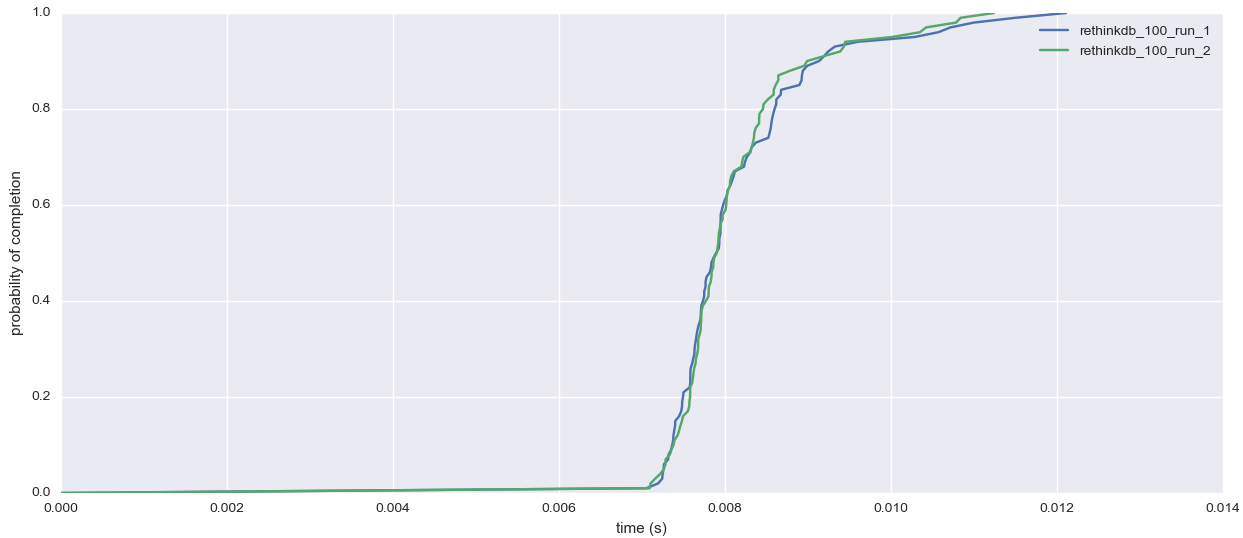
\includegraphics[width=0.8\paperwidth]{results_rethinkdb_100_mass.png}}
  \caption{RethinkDB: 100 run.}
\end{figure}

\begin{figure}[H]
  \makebox[\textwidth][c]{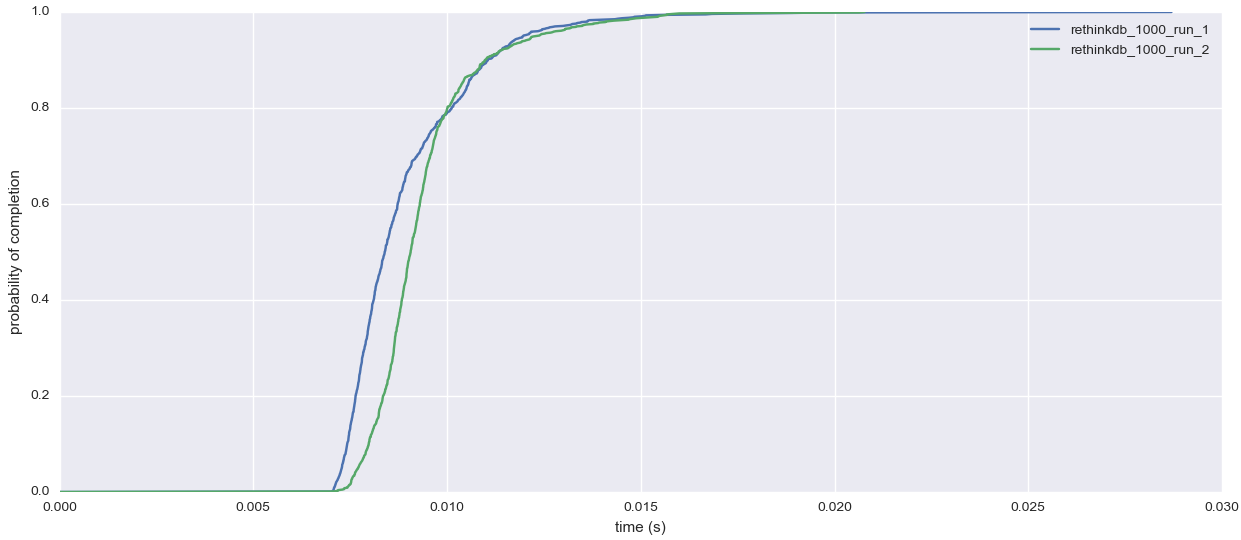
\includegraphics[width=0.8\paperwidth]{results_rethinkdb_1000_mass.png}}
  \caption{RethinkDB: 1000 run.}
\end{figure}

\begin{figure}[H]
  \makebox[\textwidth][c]{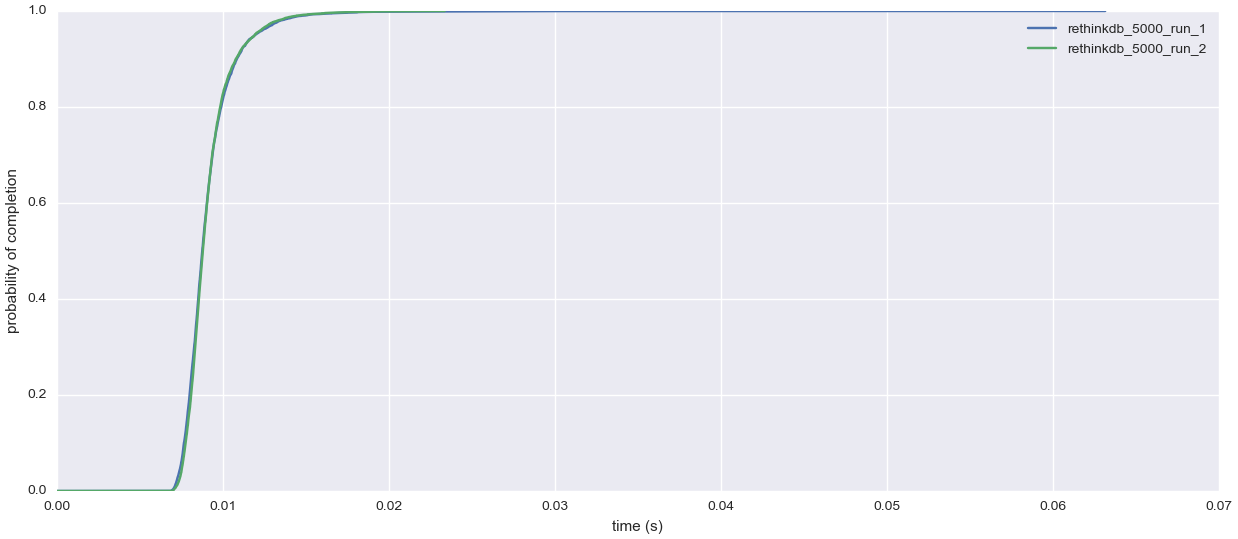
\includegraphics[width=0.8\paperwidth]{results_rethinkdb_5000_mass.png}}
  \caption{RethinkDB: 5000 run.}
  \label{rethinkdb_stable}
\end{figure}

\begin{figure}[H]
  \makebox[\textwidth][c]{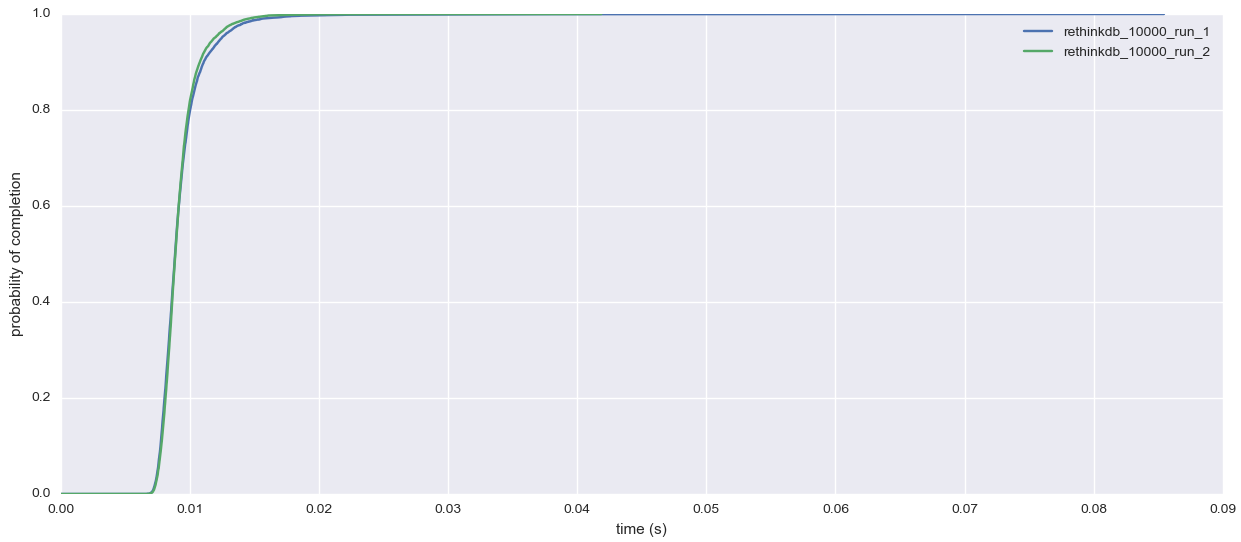
\includegraphics[width=0.8\paperwidth]{results_rethinkdb_10000_mass.png}}
  \caption{RethinkDB: 10000 run.}
\end{figure}

The parameter has been validated also on every other consensus algorithm. Figure \ref{paxos5000} shows the test on Multi-paxos.

\begin{figure}[H]
  \makebox[\textwidth][c]{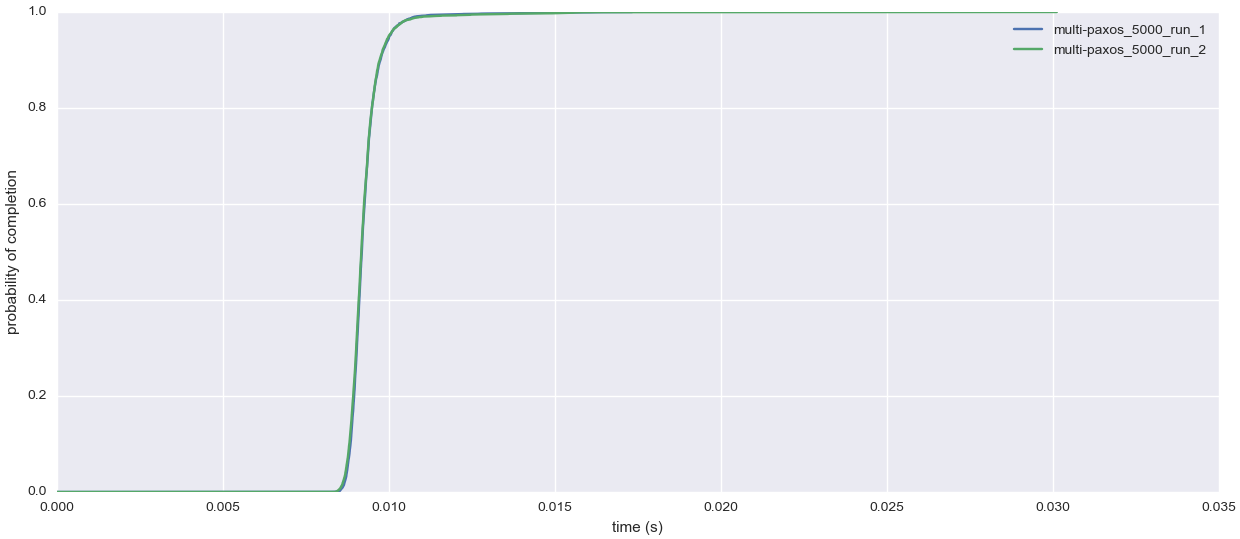
\includegraphics[width=0.8\paperwidth]{results_paxos_5000_mass.png}}
  \caption{Multi-Paxos: 5000 run.}
  \label{paxos5000}
\end{figure}

\section{Choosing the cluster size}
Another parameter to be fixed in advance has been the number of nodes composing the cluster. An upper bound of 8 has been set due to Compute Engine that doesn’t allow free-trial users to create more instances at the same time in the same region. Therefore, the value 5 has been chosen because it is reasonable enough for the majority of real distributed systems. Moreover, tests have been made to ensure that the performances on 5 nodes are not that far from the ones obtained on different size of the clusters. This has been investigated also for Multi-paxos, leading to very similar results. 

\section{Test suite description}
This section describes in depth each test in the suite. They can be divided into the following different main areas: gold standard, symmetric scenarios, asymmetric scenarios, Raft vs Paxos and Raft vs Raft.

\subsection{Gold standard}
This represents the baseline performance metric used as a guide to understand all the other results, providing insights on what to expect from every implementation. As explained before, these tests do not involve any change in the network layer.

\begin{figure}[H]
  \makebox[\textwidth][c]{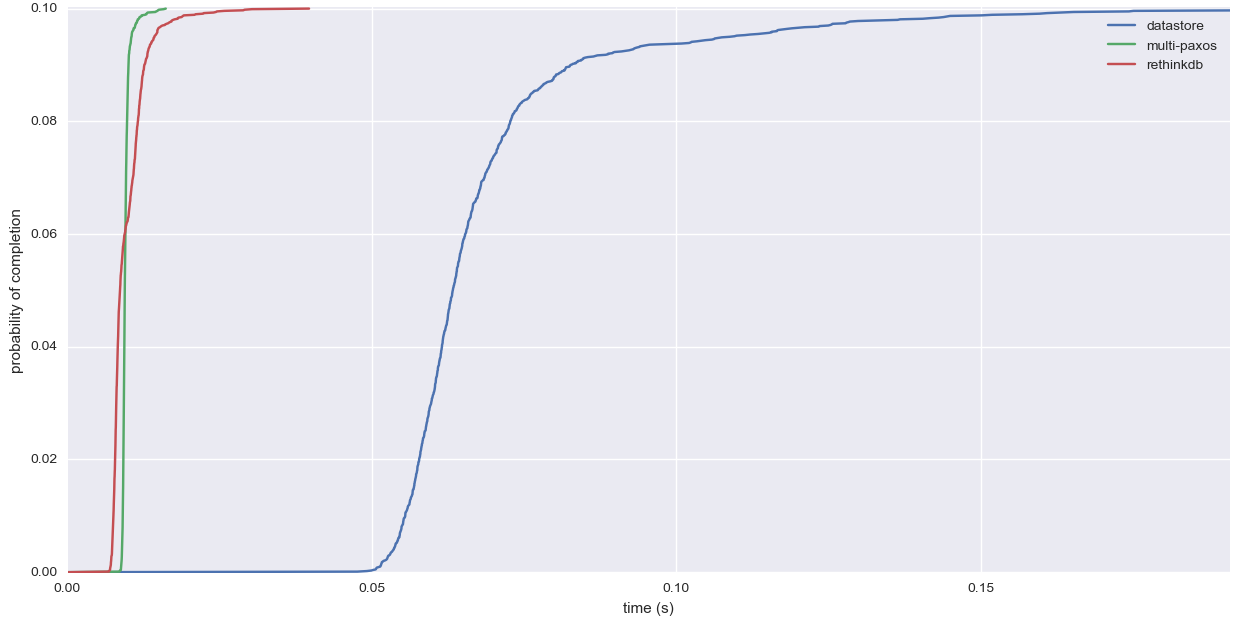
\includegraphics[width=0.8\paperwidth]{results_mass_3.png}}
  \caption{Datastore vs Multi-Paxos vs RethinkDB: cumulative density function comparison.}
\end{figure}

\begin{figure}[H]
  \makebox[\textwidth][c]{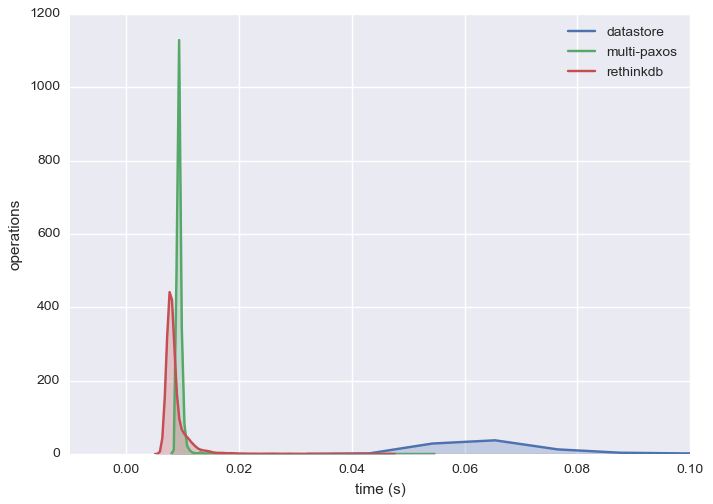
\includegraphics[width=0.6\paperwidth]{results_distribution_3.png}}
  \caption{Datastore vs Multi-Paxos vs RethinkDB: probability density function comparison.}
\end{figure}

The figures above show both the CDFs and the distributions functions of the chosen implementations. It is possible to notice how Datastore performs significantly worse than the other two algorithms and has the largest variance in the execution time. These results may be due to the fact that Datastore is not customizable by the user at will, implying that it is not possible neither to know the number of nodes the physical cluster is composed of nor to control the network traffic between them. Its execution time is approximately four time slower than the others, but it’s likely that the values stored on Datastore are replicated across Google data centers around the world on a huge amount of nodes.\\
A similar experiment has been executed in the pseudo-distributed mode. The results shown in figure \ref{local_standard} demonstrates how PySyncObj is significantly slower than every other implementations. Moreover, Multi-paxos seems to be slower than RethinkDB in this test, conversely to what shown in the previous experiment in the cloud. This is probably caused by the CPU-intensive nature of the implementation, whose effect is mitigated when nodes resides on physically different machines. On the contrary, on the local cluster all the nodes compete for the same CPU, thus mutually slowing themselves.

\begin{figure}[H]
  \makebox[\textwidth][c]{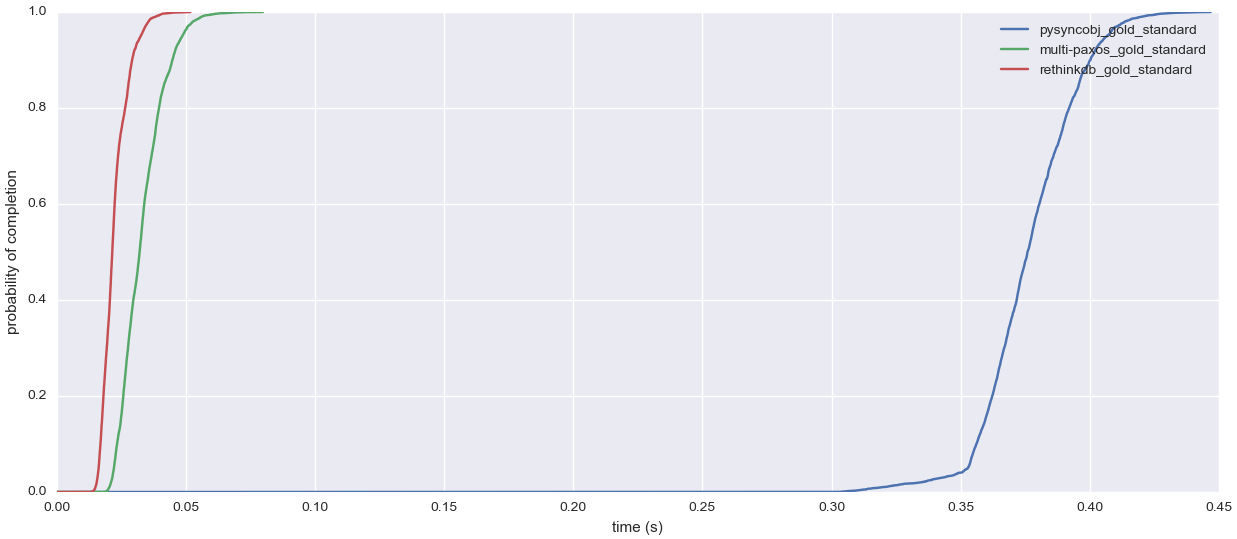
\includegraphics[width=0.8\paperwidth]{results_mass_4.png}}
  \caption{PySyncObj vs Multi-Paxos vs RethinkDB: cumulative density function comparison.}
  \label{local_standard}
\end{figure}

\begin{figure}[H]
  \makebox[\textwidth][c]{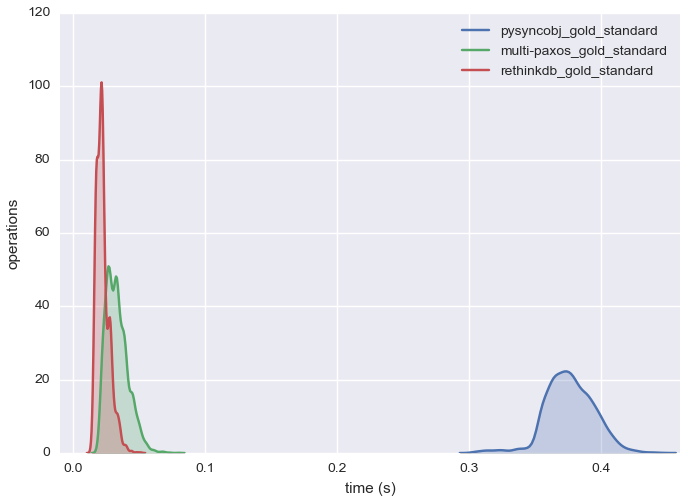
\includegraphics[width=0.6\paperwidth]{results_distribution_4.png}}
  \caption{PySyncObj vs Multi-Paxos vs RethinkDB: probability density function comparison.}
\end{figure}

\subsection{Symmetric scenarios}
These tests shows how the system performance degrades while increasing problems on the network in a homogeneous manner. They have been specifically crafted to give the consensus algorithm hard times in replicating data between the nodes. Every distributed algorithm relying upon message passing for communication should be affected by these changes. The completed tests are the following:

\begin{itemize}
    \item packet delay: every node in the cluster transmits with a certain delay its packets, both ingoing and outgoing. The tested delay are 10 ms, 15 ms and 20 ms.

    \begin{figure}[H]
      \makebox[\textwidth][c]{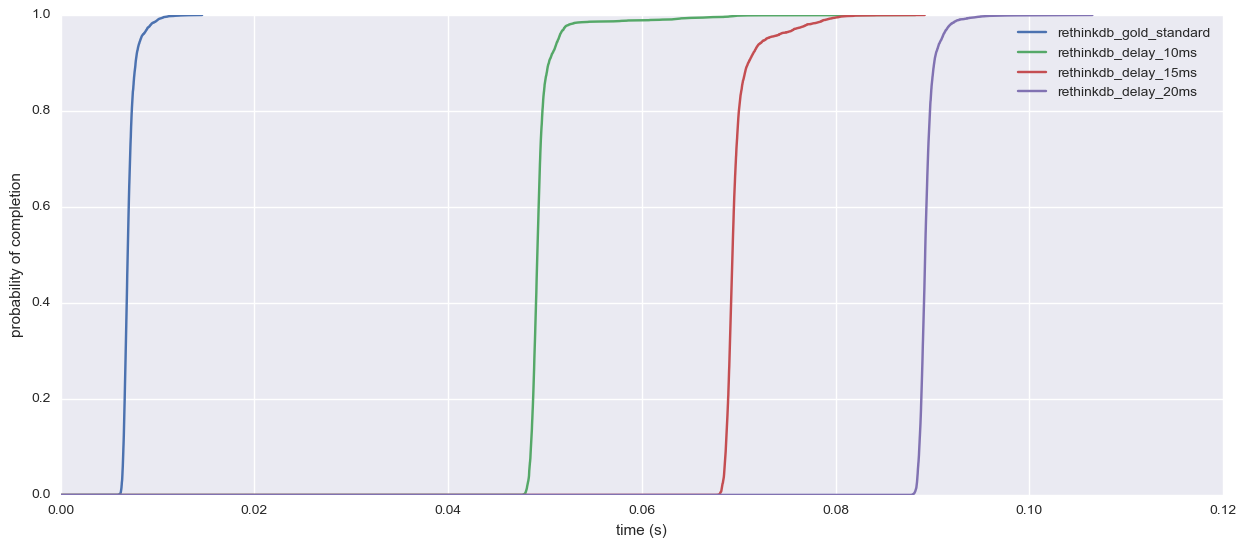
\includegraphics[width=0.8\paperwidth]{results_delay_mass_5.png}}
      \caption{RethinkDB: cumulative density function with delay.}
      \label{delay}
    \end{figure}

    \begin{figure}[H]
      \makebox[\textwidth][c]{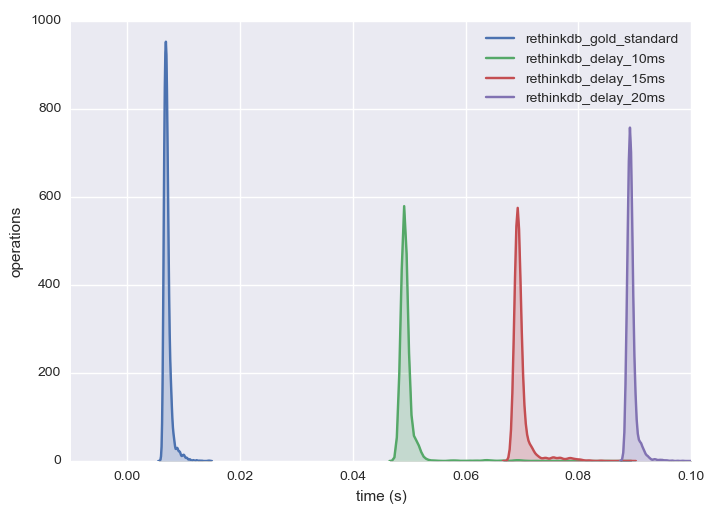
\includegraphics[width=0.6\paperwidth]{results_delay_distribution.png}}
      \caption{RethinkDB: probability density function with delay.}
      \label{delay_distr}
    \end{figure}

    \item packet loss: every node in the cluster loses a certain percentage of packets, both ingoing and outgoing. The tested percentages are \(2\%\), \(4\%\) and \(6\%\) with a uniform distribution.

    \begin{figure}[H]
      \makebox[\textwidth][c]{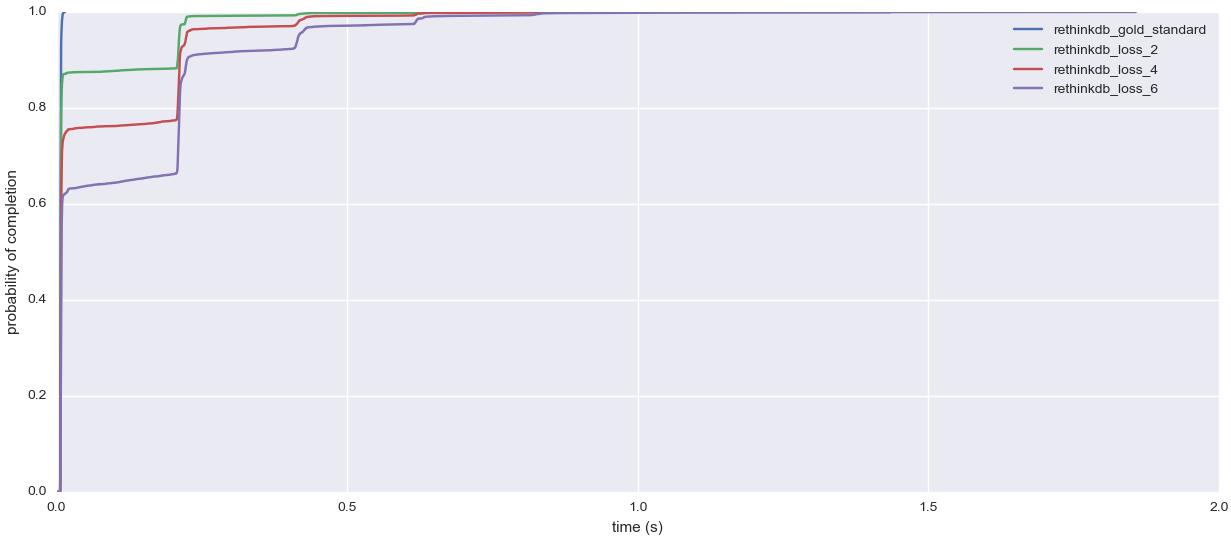
\includegraphics[width=0.8\paperwidth]{results_loss_mass.png}}
      \caption{RethinkDB: cumulative density function with loss.}
      \label{loss}
    \end{figure}

    \item packet corruption: every node corrupts a certain amount of packets, both ingoing and outgoing. The tested percentages are \(2\%\), \(4\%\) and \(6\%\) with a uniform distribution.

    \begin{figure}[H]
      \makebox[\textwidth][c]{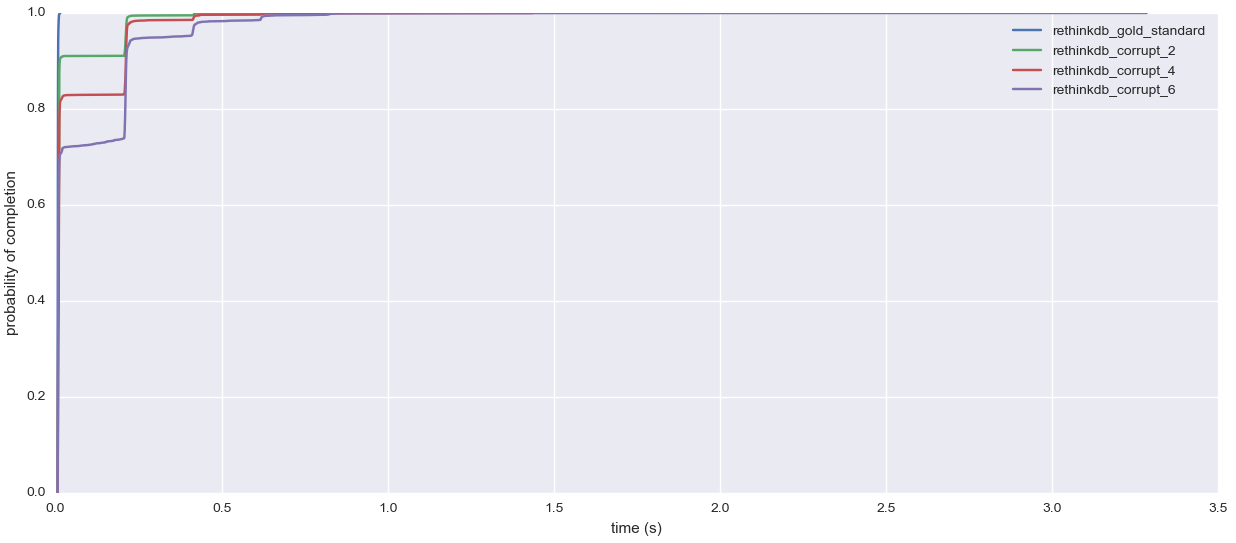
\includegraphics[width=0.8\paperwidth]{results_corruption_mass.png}}
      \caption{RethinkDB: cumulative density function with packet corruption.}
      \label{corruption}
    \end{figure}

    \item packet inversion: every node randomly reorders \(50\%\) of the packets, both ingoing and outgoing and sends the other half with a certain delay. The chosen delays are 10 ms and 20 ms.

    \begin{figure}[H]
      \makebox[\textwidth][c]{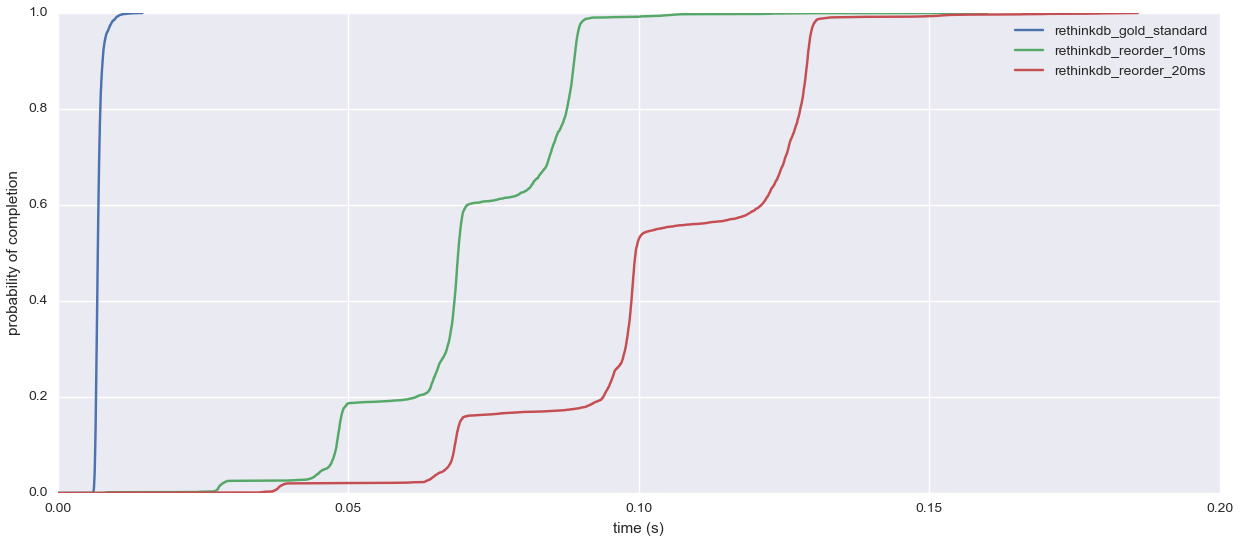
\includegraphics[width=0.8\paperwidth]{results_reorder_mass.png}}
      \caption{RethinkDB: cumulative density function with packet reordering.}
    \end{figure}
\end{itemize}

In the figures \ref{delay}, \ref{loss} and \ref{corruption} the trend of the CDFs clearly shows how introducing these network issues influences the time the system needs to reach consensus in a proportional manner. This effect can be seen by looking at the shift of the lines along the x axis towards higher values of elapsed time. The proportionality factor can provide some insights on the number of messages that are exchanged by RethinkDB to reach consensus. As it can be seen in the figure \ref{delay_distr}, with a 10 ms delay the consensus is reached on average in 50 ms. By increasing the delay of only 5 ms, the consensus time increases to 70 ms. The average number of sequential messages exchanged by RethinkDB can be thus computed with the following formula:

\begin{align*}
  0.50 - 0.10*n &= 0.70 - 0.15*n \\
  n &= 4
\end{align*}

The packets loss graph shows different information. The first gap underlines the effect of one packet loss on the consensus algorithm. The height of each gap represents the probability of not losing more than one packet and it represents an index of the minimum number of messages (not necessarily in sequence) that the underlying algorithm needs to exchange to reach consensus. In fact, increasing loss percentages decreases the probability of reaching consensus (red and purple lines). The second gap, similarly, represents the loss of two packets and so do the successive ones. The distance on the x axis between two gaps represents the time that RethinkDB takes to recover from a packet loss and it is constant on each gap (\(\sim0.2s\)).\\
A similar behaviour can be seen on the packet corruption graph. The main difference from the packet loss is that corruption seems to affect less the protocol, since consensus probabilities are slightly higher. This trend can be due to the fact that one bit corruption has a non-zero probability of leaving the TCP packet intact from an application level point of view.\\
The reordering graph, on the other hand, shows a different behaviour which seems to be the combination of both packets loss and delay.

\subsection{Asymmetric scenarios}
These tests show how the system performance degrades when the network faces problems on a specific subset of nodes. Adversarial network conditions have been applied only to some nodes to model new network situations, common in distributed systems. The tests that have been completed are the following:

\begin{itemize}
    \item faulty network cards: 1 random bit of ingoing and outgoing packets gets corrupted with a probability of 0.1. One at a time, every node of the cluster suffers this condition.

    \begin{figure}[H]
      \makebox[\textwidth][c]{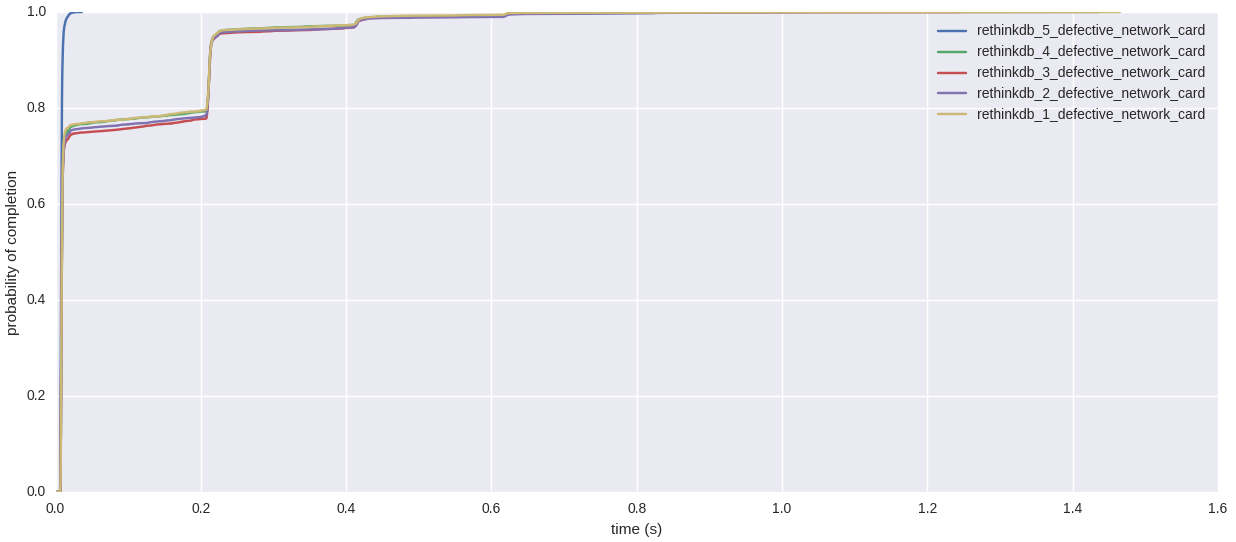
\includegraphics[width=0.8\paperwidth]{results_rethinkdb_broken_network_card_mass.png}}
      \caption{RethinkDB: cumulative density function with broken network cards.}
      \label{broken_nic}
    \end{figure}

    \item partitions: some links that connect a group of the nodes in the cluster to the others are slowed down. This situation simulate a distributed system whose nodes are logically partitioned into two different regions. In this way the intra-partition communication is slow, but, at the same time, the inter-partition communication is left unchanged.

    \begin{figure}[H]
      \makebox[\textwidth][c]{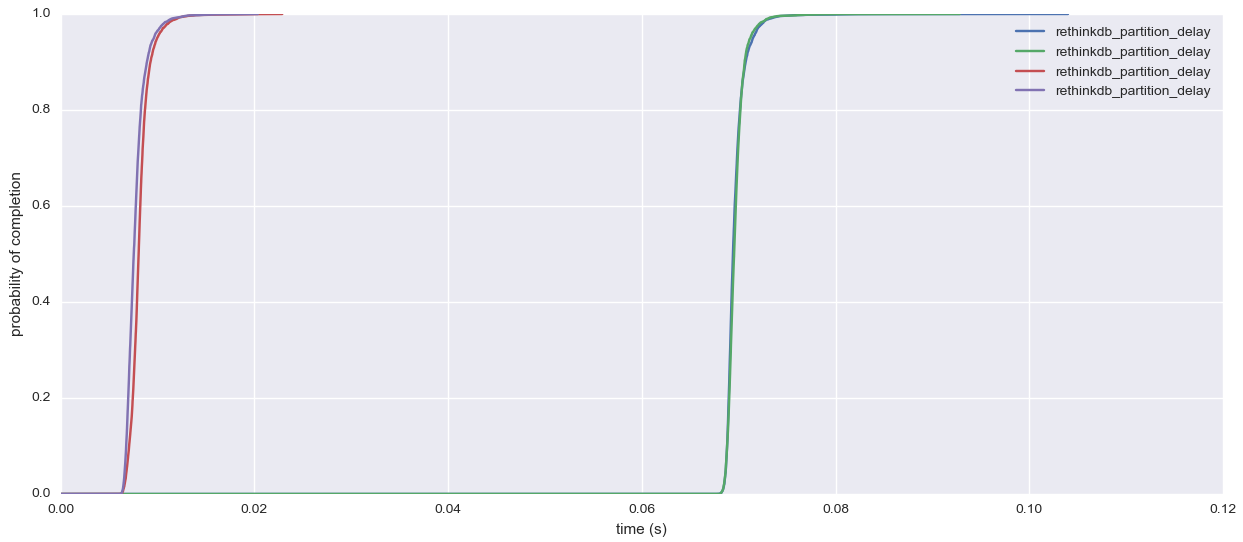
\includegraphics[width=0.8\paperwidth]{results_rethinkdb_slow_links_between_regions_mass.png}}
      \caption{RethinkDB: cumulative density function with partitions.}
      \label{partitions}
    \end{figure}
\end{itemize}

The results in figure \ref{broken_nic} shows two different behaviours. If the node having the problem is one which is not necessarily involved in the majority to reach consensus, the consequences are negligible (blue curve). On the other hand, if the faulty network card is the one of a node which is actually needed to obtain consensus, the performances deteriorate (all the other lines).\\
figure \ref{partitions} explains how the Raft algorithm responds to a logically-partitioned cluster with groups made of 2 and 3 nodes respectively. More in detail:

\begin{itemize}
    \item if the leader and a majority of the nodes are together, the algorithm is not delayed at all, since nobody in this partition needs to communicate with another node through a slow link. This situation is represented by the purple and the red lines on the left side.
    \item if the leader needs to contact any node afflicted by a slow link, it has to wait for him to respond and the overall performances are clearly worse (green and blue lines on the right). 
\end{itemize}

\subsection{Raft vs Paxos}
This test is thought to compare the two consensus algorithms and show which of them suffers more packets delay, which is probably the most frequent issues on real systems.

\begin{figure}[H]
  \makebox[\textwidth][c]{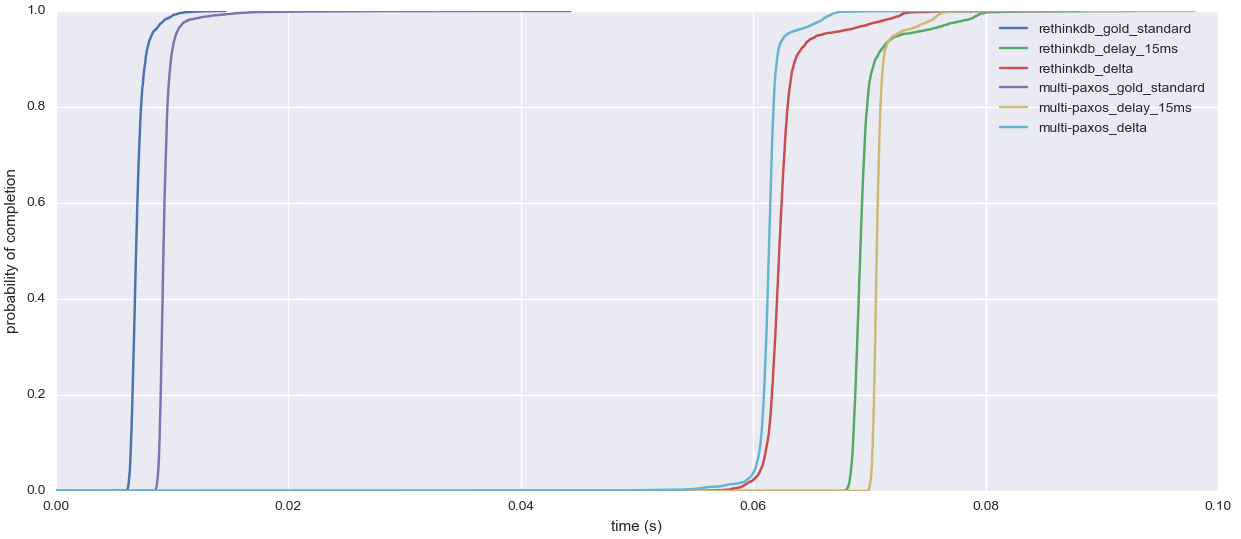
\includegraphics[width=0.8\paperwidth]{results_delay_mass_7.png}}
  \caption{RethinkDB vs Multi-Paxos: cumulative density function comparison with delay.}
\end{figure}

The figure above illustrates how Multi-paxos performs slightly better than RethinkDB if the delay is quite small (15 ms). This can be easily noticed by looking at the two curves in the middle, showing the difference between the gold standards and the delayed executions, where Multi-paxos (light blue) is on the left with respect to RethinkDB (red).

\subsection{Raft vs Raft}
Different implementations relying upon the same consensus algorithms are compared in order to demonstrate how RethinkDB clearly outperforms PySyncObj. In this way it is possible to see how a commercial product is orders of magnitude better than its counterpart from any point of view.

\begin{figure}[H]
  \makebox[\textwidth][c]{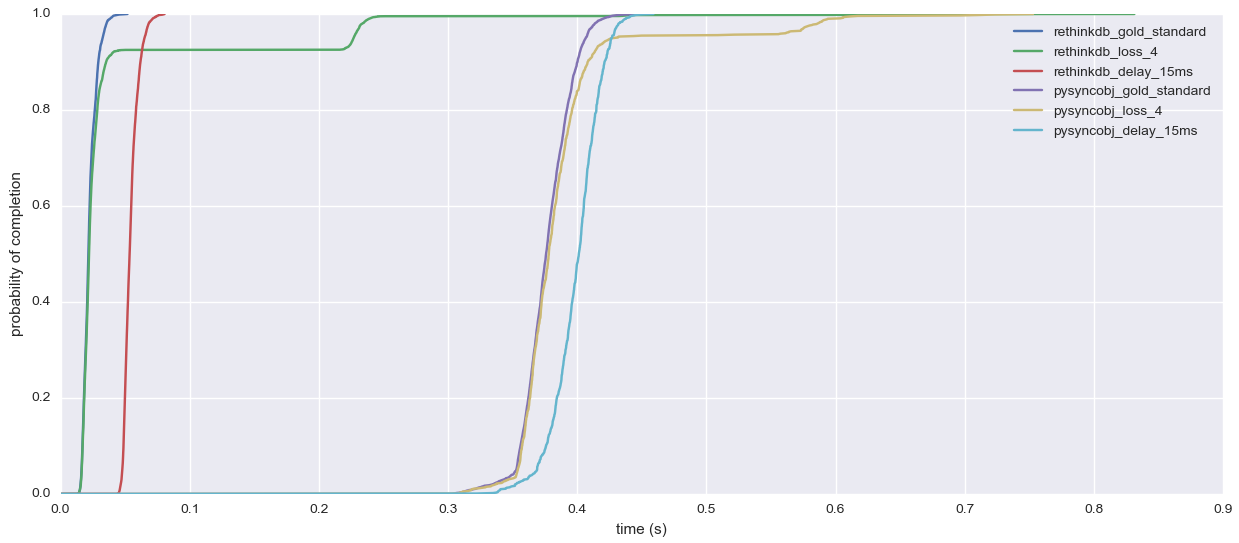
\includegraphics[width=0.8\paperwidth]{results_mass_raft.png}}
  \caption{RethinkDB vs PySyncObj: cumulative density function comparison with delay and loss.}
\end{figure}
%!TEX root=../report.tex
\chapter{Conclusion}\label{chp:conclusion}

Distributed algorithms are typically tested validating all the possible interactions between a set of nodes. This task is usually performed simulating different processes on local machines or by using different machines in a network. This phase typically requires many efforts, both for the wide range of scenarios produced by interleaving executions and for the difficulties in debugging remote machines. The testing approach proposed in this work is different since it directly manipulates the network underlying the system rather than acting on individual nodes. This solution allows the tester to model many different situations with little effort. The black-box approach suits this paradigm and such kind of tests can be easily performed using the developed platform. Even if network modifications affect the lower level message exchange, many useful insights on the upper application level logic can be inferred.
For the purpose of this work, the platform has been used to test different implementations of Raft and Paxos consensus algorithms. The tests performed on Multi-paxos show it favours a distributed environment rather than a pseudo-distributed one. This is probably due to the CPU-intensive nature of this particular implementation. Furthermore, Multi-paxos is not performing failovers in an efficient way after a period of serious problems on the network.\\
RethinkDB seems to be the overall winner, even though other implementations reach slightly better results in some tests. This may be due to internal optimizations, but investigating them is out of the scope of this work. The product proved to be very well implemented and very robust, being capable of performing disaster recovery in a small amount of time. Moreover, RethinkDB is highly customizable and this flexibility well suits different users’ requirements.\\
Finally, as expected, commercial products turned out to be much better than their counterparts, especially from the safety point of view.

%\pagestyle{plain}
\renewcommand{\chaptermark}[1]{\markboth{{\appendixname}\ \thechapter.\hspace{1em}#1}{}}

%\appendix
%\input{sections/appendix.tex}

%\clearpage
%\addcontentsline{toc}{chapter}{References}
%\bibliographystyle{plain}
%\bibliography{bibliography}

\end{document}